\vspace{10pt}

{\centering\subsection*{何以萱:放风筝}}

\addcontentsline{toc}{subsection}{何以萱:放风筝}

\renewcommand{\leftmark}{何以萱:放风筝}

\begin{figure}[htbp]

\centering

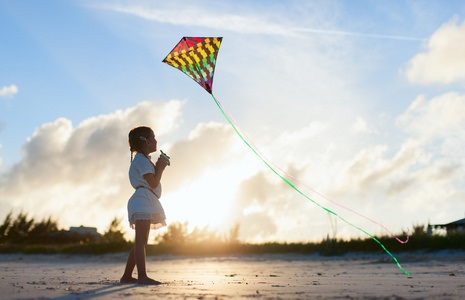
\includegraphics[width = .5\textwidth]{./ch/27.jpg}

\end{figure}



周六的上午,天气晴朗,春风拂面,正是放风筝的好天气。我和好朋友微微、小强来到公园里准备放飞我们珍藏的大风筝。

呵,公园里的小山坡上已经聚集了不少放风筝的人了。我们头顶上飞舞着各式各样的风筝,有蜈蚣、有苍蝇、有金鱼………看,远处那个小弟弟刚刚放起了彩色风筝给他的爸爸妈妈欣赏呢!小强赶紧拿起自己的风筝对我说:“小明,你来放线,我举着风筝,好吗?”“好啊!”我接过线轴。小强迎着风站好,高高举起风筝,我一只手握着轴,一只手轻轻地放线,一点点跑起来。线越放越长,我越跑越快,小强高兴极了,大声喊着:“小明,再快点儿,燕子就要飞起来啦!”微微抱着他那漂亮的蝴蝶风筝,笑眯眯的快步跟着我,悄悄对我说:“小明,一会儿也要帮我放哟!”

不一会儿,我们的沙燕和蝴蝶都飞上了天空,它们迎着春风越飞越高,我们的欢呼声也越来越高。明年我们还要一起放风筝,放飞我们的快乐!





\vspace{10pt}



作者:三(3)班 何以萱



指导老师:何业平



投稿:2021年5月10日



发表:2021年5月10日




                



\vspace{10pt}

\hline



